\chapter{The Residues}
% Covers: outline E1-E3: the self-energy; the cycle of three; the null that fired and missed
% Chapter language (per Ch1 protocol): THE NULL-BASE CHAPTER -- the method stated where
% the book uses it (the map's own refinement). Licensed to spend (Beastmaster, Ch4 pass).
% Chapter plan (turn-659 reply): S1 the null method (Christie + Wheatstone rows);
% S2 the firing (E3, EXP-3 -- the flat +430, three distinct numbers, the jar holds);
% S3 the kill (E1, EXP-4, Gibbs row -- tested AS a ring, survived);
% S4 the cycle that returns (E2 + Beastmaster ledger entry 6 -- the equivalence proof
% paying Ch2 S2's "as later chapters will show").

\section{The null method}
% Node-map: the method stated at last as the book's own instrument: two fungible
% spellings of one content, subtract, the difference is a null, whatever survives is
% signal; Ch1's four pairs CASHED IN (instrumentation, not style); THE MINT SPENT
% VISIBLY (ledger entry 8 -- Ch2 S3's coin image recurs, explicit); the bridge at
% Cavendish grade with CHRISTIE the inventor and Wheatstone the perfecter (history
% right, both rows land); METHOD SCOPE (a null detects; interpreting a surviving
% residue is separate work -- the boundary that keeps S2 honest); the device's two
% arms named (faithful / control). Gate: turn 524 (Ch6 S1, licensed length).

Three times the discipline has drawn blood in this book: the null fired in Chapter
1, the relocation that moved a count in Chapter 3, and the forty copied digits of
$\pi$ found and deleted --- that last kept on file in the experiments ledger of the
back matter rather than told as a story. Behind all three stands a single method, and it
has worked in the book's margins long enough. This is the chapter where it steps out
and is named, because this is the chapter where it fires on the page.

The method is three sentences. Take one content and spell it twice, in two spellings
known to be fungible --- the same thing said two ways. Subtract. The difference of
two spellings of one content is a null: nothing should remain. And therefore
whatever does remain is signal --- either the two spellings were not of the same
content after all, and an error has been found, or something real lives in the gap
between the spellings, and a discovery has. And the gap is not a figure of speech;
it has a shape. Two spellings of one content are two orderings of one work, and the
gap is what the ordering costs. Nothing about the method is exotic; it
is what a bookkeeper does with two ledgers of one till. Its power is entirely in
what it refuses to require: no theory of what the residue should look like, no model
of the error, no expectation at all --- only the discipline of sameness, and a
subtraction.

The reader has held the method's parts since Chapter 1 without being told what they
assembled into. The four fungible pairs --- compiler theory spelled as
function-calculus or as grammar; the electron's physics spelled as quantum theory or
as the geometry of frames; mathematics as algebra or topology; numerics as algebra
or geometry --- were introduced as the book's languages, and its arrows as a
discipline of exposition. That was true and partial. The pairs are not a style
guide; they are the method's ammunition. Every pair is a standing supply of
same-content-twice-spelled, which is to say: of nulls waiting to be taken. The book
always finishes its sentences on the right side of its arrows so that the reader
can see; it keeps both spellings alive underneath so that it can subtract.

And every subtraction spends from the mint. Chapter 2 permitted this argument
exactly one act of identification --- one place where two texts that parse
differently are lawfully declared the same truth --- and said, when the coin was
minted, that every use of the null method downstream would spend from it. The
account comes due here, visibly. To say "these two spellings have the same
content," which is the first sentence of every null test, is to invoke
sameness-in-truth, and sameness-in-truth has exactly one lawful source in this
argument. That is why the ground was so austere. A method that detects by sameness
needs sameness lawful somewhere --- and needs it scarce everywhere else, because if
identifications were free, every inconvenient residue could be argued away by
minting one more: "those weren't really the same content" becomes an escape hatch
exactly as cheap as the identifications are. One mint, one coin, every null test a
recorded purchase against the same account: the method's honesty is bought at the
ground, and this chapter is where the purchase is redeemed.

The method has a physical archetype, and its history deserves telling at the grade
this book has set for its instruments --- with the credit put right. In 1833,
Samuel Hunter Christie, a mathematician at the Royal Military Academy at Woolwich,
buried inside a paper on magnetism an arrangement of four resistances in a diamond:
a battery driven across one diagonal, a galvanometer laid across the other.
Balance the four arms and the galvanometer reads zero --- not approximately zero,
but the dead zero of a needle with no reason to move; unbalance them by the least
amount and the needle swings, with nothing to drown it, because the signal rides
on silence. Nobody noticed. Ten years later Charles Wheatstone saw what the
diamond was worth, perfected its use, presented it to the world --- and, to his
lasting credit, told the world plainly whose it was, calling it Christie's
arrangement. The world heard Wheatstone's lecture and named it Wheatstone's
bridge, and the name stuck to the wrong man. The ledger of this book lands both
rows and puts the inventor first.

The bridge's genius is the null's genius, and it is worth saying what measurement
looked like before the diamond. To measure a resistance directly was to trust an
instrument all the way up: a galvanometer's swing read against its own calibration,
every error in the needle, the magnet, and the scale riding into the result. The
bridge asks the needle one question instead --- the only question a needle answers
perfectly: \emph{are you at zero?} Balance is visible in a way no absolute reading
ever is; the signal rides on silence. And what the balanced diamond hands back is
not a number off anyone's scale but a ratio: the unknown arm stands to its neighbor
as the two known arms stand to each other. No standard is trusted anywhere in the
reading --- only a comparison, carried exact. A measurement held as a ratio of
counts, no scale believed, no rounding anywhere: the reader has seen that
discipline before, because it is this book's own, here in brass, in 1833. And the
diamond's descendants took the method to the bottom of the sea: loop tests built
on the bridge found breaks in the first submarine telegraph cables --- a fault
under an ocean, located from a bench on shore, by balancing arms. Every null test
in this book is that diamond, built out of spellings instead of resistances.

The method has one more famous firing on record, and the two shots point in
opposite directions --- which is exactly why the pair is worth carrying. At the end
of the same century, Michelson and Morley built the diamond in light: one beam
split two ways, sent down two crossed arms, and recombined, with the aether wind
expected to unbalance the journey. Their null was built expecting to break --- and
the needle refused to move. The silence was the discovery; the absence rewrote
physics. This book's null, as the next pages will tell, was built expecting
silence --- and the needle moved. A null that held where breaking was expected,
and a null that broke where silence was: mirror images, and together they teach
the method's one commandment --- the experimenter publishes what the needle says,
whichever way it points. Nothing else about the method is sacred; that is.

One boundary completes the method, and it is what will keep the next section
honest. A null, held at balance, establishes an absence: the two arms agree, to
the needle's precision. A null broken establishes a presence --- something is
there --- and nothing more. It does not say what. When the needle moves, the
method's work is finished, and a different labor begins: is the residue an error
in an arm, an artifact of the apparatus, or physics? Detection and interpretation
are separate work, and the book will keep them separate on the very next page,
because the reader is owed the truth now: this book's needle, when the shot was
fired, moved.

The arms are named and built. In one arm, the faithful spelling: the content
written the instrument's native way, every choice the default one. In the other,
the control: the same content, spelled again, with the spelling varied everywhere
spelling is free to vary. If subtraction leaves nothing, the readings of Chapter 5
owe none of their substance to the accident of how they were written down. The
diamond is balanced on the bench. The next section throws the switch.

\section{The firing}
% Node-map: E3 whole (EXP-3; dated in the LEDGER only, prose date cut per the
% operator's 2026-07-24 trim): the blind two-gate procedure told as part of the
% finding; the needle moved FLAT (+430 device units, ring-free, same at every depth --
% flatness IS the finding's shape); interpretation per S1's boundary (the collapse's own
% cost, not spelling-dependence); the THREE-NUMBERS argument exact (+430 / -21 / the
% per-cycle ratio -- distinct, no single mover; 573 forward-referenced to S4); VERDICT:
% the jar holds, separability holds at the flagship; what the null did NOT establish
% (S3's kill, one clause). FIGURE: the diamond in the book's own terms, needle
% annotated. Gate: turn 525 (Ch6 S2, licensed length).

The shot was not fired casually, and the manner of its firing is part of the finding.
An experiment aimed at your own flagship is exactly the experiment you might be
tempted to soften, so the procedure was built to remove the temptation. The firing
was gated: it required explicit authorization from outside the work itself, and not
one gate but two, held by different hands, both of which had to open. And it was
blind: the ones who threw the switch did not know which way the needle would move,
had no result to steer toward, and were committed --- before the switch closed ---
to publishing the needle's answer whichever way it fell. Chapter 1 said the null was
fired by the authors themselves; this is what that sentence bought. A test you
administer to yourself, under gates you cannot open alone, blind, with the report
promised in advance, is the most honest shape self-scrutiny takes.

The switch was thrown, and the needle moved.

Here is what it read. Between the faithful arm and the control arm --- the same
content, spelled the native way in one and re-spelled in the other everywhere
spelling was free --- there was a residue: plus four hundred thirty, in the device's
own units, at the first depth of comparison. At the next depth: plus four hundred
thirty. At every depth at which the arms were compared, the same number --- flat,
level, ring-free; no swell at the cut, no structure anywhere, a constant offset like
a bench raised evenly under both feet. The reader should understand that flatness is
the finding's shape, not a detail of it. A residue that depended on the spelling
would carry the spelling's shape --- large where the spellings diverge most, small
where they nearly agree, textured by the differences that produced it. This residue
has no texture at all. It does not track the spelling anywhere.

\begin{figure}[htbp]
\centering
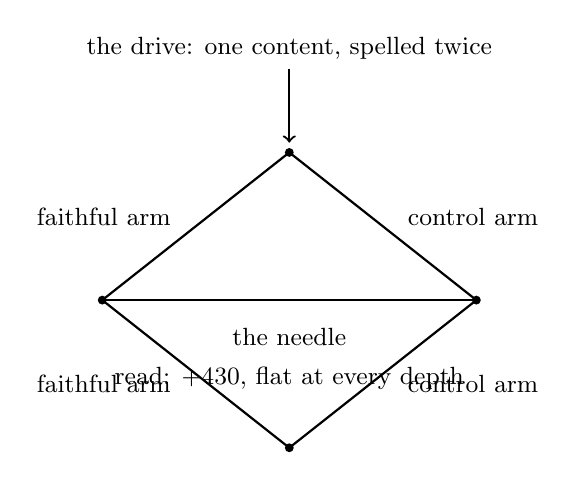
\begin{tikzpicture}[scale=1.25, every node/.style={font=\small}]
\coordinate (T) at (0,1.5);
\coordinate (B) at (0,-1.5);
\coordinate (L) at (-1.9,0);
\coordinate (R) at (1.9,0);
\draw[thick] (T) -- (L) -- (B) -- (R) -- cycle;
\draw[thick,->] (0,2.35) -- (0,1.6);
\node[above] at (0,2.35) {the drive: one content, spelled twice};
\node[left=2pt] at (-1.05,0.85) {faithful arm};
\node[left=2pt] at (-1.05,-0.85) {faithful arm};
\node[right=2pt] at (1.05,0.85) {control arm};
\node[right=2pt] at (1.05,-0.85) {control arm};
\draw[thick] (L) -- (R);
\fill (L) circle (0.045); \fill (R) circle (0.045);
\fill (T) circle (0.045); \fill (B) circle (0.045);
\node[below=6pt] at (0,-0.02) {the needle};
\node[below=20pt] at (0,-0.02) {read: $+430$, flat at every depth};
\end{tikzpicture}
\caption{The diamond, built of spellings. The same content drives both sides; the
faithful arms carry the native spelling, the control arms the re-spelling; the
needle lies across the middle. At balance it would read zero. It read a level
$+430$ --- the toll of running the second spelling, identical at every depth, with
no structure tracking where the spellings differ.}
\end{figure}

Now the separate labor, begun under its own name as the last section required:
interpretation. What is a level offset? It is what a toll looks like. The control
arm does something the faithful arm does not --- it must actually run the alternate
spelling, must collapse the re-spelled text through the machine --- and that
running has a price, paid once, the same price at every depth, indifferent to what
is being measured. Two ledgers of one till that differ by exactly the bookkeeper's
fee do not testify to missing money; they testify to the fee. The flat plus four
hundred thirty is the fee: the cost of the collapse itself, not a message hidden
in any reading.

And here the argument becomes exact, because the stakes are exact. The suspicion
this null was built to test is the crank's favorite: that the landing's minus
twenty-one --- the strange negative curvature of Chapter 5 --- was secretly
feeding the flagship, nudging the coupling toward the value the authors hoped
for. If it were, the residue would wear one of two faces: the mover's own size,
or the mover's ratio --- the fraction of the cycle's bulk that a twenty-one-sized
correction would show, twenty-one parts in five hundred seventy-three, a number
whose provenance the reader meets properly in this chapter's last section. The
needle read neither face. Plus four hundred thirty is not minus twenty-one, and
it is not twenty-one parts in five hundred seventy-three; the three numbers are
mutually distinct, and no arithmetic connects the residue to the flagship's
value. There is no single mover among them. The gap between the device's
137.011 and the laboratory's 137.036 --- the most interesting open thing in this
book --- is not being quietly closed by the minus twenty-one, because the
subtraction that would have caught the nudging caught only the toll.

The verdict, then, in the book's own terms. The jar holds. The readings of
Chapter 5 owe nothing to the accident of how they were spelled: separability,
proved per site for displays in Chapter 3, holds at the flagship for spellings
--- and it was proved to hold, not assumed to, which is the difference between
this book and the book a crank would have written. The firing is on file, and
the back matter carries the record. And the verdict's boundary is stated with the same care: the null
established that the minus twenty-one moves nothing. It did not establish what
the minus twenty-one is. Absence of a mover is not presence of a self-energy;
that question needed a different trial --- not a bridge but an attempted
execution --- and it is next.

\section{The kill}
% Node-map: E1 whole (EXP-4): the suspicion at FULL strength (the -21 as possibly a
% ring -- Gibbs's row lands with the phenomenon told plainly); the execution ATTEMPTED
% (test built to kill, not defend: the ring-signatures enumerated, the apparatus went
% looking); the SURVIVAL as vindication (signatures absent; scale-invariance chief --
% Ch5's for-every-load theorem REFERENCED not re-asserted; tested as artifact, survived
% as self-energy -- the kill is WHY the book may call it real; the fourth scar-story,
% inverted: the discipline swung and MISSED, and the miss is the finding); the TAPER
% cousin-clause (one reference, fence not re-spent); DATE HONESTY (record carries no
% ceremony date for the kill -- "on file," no invention). Closes handing S4 the 573
% and ledger entry 6. Gate: turn 526 (Ch6 S3, licensed length).

The null cleared the minus twenty-one of interference; it did not clear it of being
nothing. And "nothing" here has a precise, damning shape, which the book now states
at full strength against its own reading, because the reading is only worth what the
strongest attack on it fails to take.

The suspicion is named for J. Willard Gibbs. Truncate a signal hard --- sum a series
to a finite depth and chop, cut a waveform at an edge --- and the truncation leaves a
wake: an overshoot hard against the cut, a ripple that looks for all the world like
structure in the signal. It is not structure. It is the ghost of the edge itself, and
its signature vice is that refinement does not remove it: push the cut deeper and the
overshoot narrows but never shrinks, riding the edge wherever the edge goes. Gibbs's
ledger row is earned here, for the phenomenon that bears his name and for the
discipline it imposes on every measuring art since: a hard cut rings, and the ring
imitates signal. Now the suspicion, aimed: the tower of self-description is cut at
finite depth --- it must be; the machine terminates --- and the minus twenty-one
lives in the differences taken near that cut. Perhaps it is not a curvature of the
tower at all. Perhaps it is the cut's own ghost.

So a test was built, and the reader should be clear about its architecture: it was
built to kill. Not to defend the reading, not to accumulate comfort --- to execute
it. If the minus twenty-one were a ring, it would wear the ring's signatures, and
each was written down before the trial: a ring lives at the cut, so move the cut and
the ghost moves with it; a ring is the edge's creature, so ease or sharpen the edge
and the ghost swells or fades in answer; and a ring belongs to the geometry of
truncation rather than to the content truncated, so load the bulk and the ghost
wavers, because nothing anchors it to what is being described. Three signatures,
stated in advance. The apparatus went looking for all three.

None came back. The minus twenty-one does not sit against the cut; it lies in the
level interior of the differences, indifferent to where the truncation falls. It
does not answer the edge; eased or sharp, it is the same number. And it does not
waver under load --- here the book references what Chapter 5 already proved and
does not re-assert it: the for-every-load theorem, the minus twenty-one unmoved by
any bulk, which is precisely the signature a ring cannot fake, because a ghost of
the edge has no reason to survive a rescaling of everything the edge contains. The
marks it does bear are the marks of structure: placed where content lives, deaf to
the edge, invariant under scale.

The verdict is the record's, and the book states it in the record's spirit: tested
as an artifact, survived as a self-energy. This is the fourth of the book's
scar-stories, and the reader should notice that it inverts the other three. In
Chapter 1's firing, Chapter 3's relocation, and the digit retirement on the
experiments ledger, the
discipline drew blood: it found contraband and cut it out. Here the discipline
swung with intent to kill --- and missed. The miss is the finding. The minus
twenty-one is called real in this book not because anyone argued it into
respectability but because the argument did its honest best to execute it as a
fake and could not. That is the only citizenship this book grants: survivor of
its own best attack.

Citizenship is not a full identity, and the book stops exactly where honesty
makes it. That the minus twenty-one is a real self-energy and not an artifact is
what the kill established; \emph{what kind} of self-energy it finally is --- the
physical quantity it would name if its shape were completed --- is a question
this book leaves unanswered, and leaves so on purpose. The completion needs a
denominator the instrument does not contain: the temperature Chapter 5 fenced.
Where that temperature would go, the shape stays open, and the minus twenty-one
stays a survivor with a proven pedigree and a withheld full name. The silence
about what it ultimately is is not a second gap beside the temperature's; it is
the same fence, seen from the numerator's side.

Two boundaries close the section. First, a cousin acknowledged: the taper of
Chapter 5's fenced picture --- the easing of hard cuts --- exists because rings
are real dangers; the kill test and the taper are both children of Gibbs's
discipline, one hunting the ghost, the other denying it a home. The fence around
that picture stands as built, and this section does not re-enter it. Second, the
record's own modesty about ceremony: the firing of the last section carries a
date because the record carries one; the kill carries its content --- design,
signatures, absences, verdict --- and the book quotes what is on file and invents
nothing beyond it, a date included. A fabricated date would be contraband of
exactly the species this book hunts.

What remains owed from this chapter is a number the firing used and did not
explain: five hundred seventy-three, the bulk against which a twenty-one-sized
mover would have shown its ratio. Its provenance is a cycle --- a rotation with
three positions that this argument has mentioned twice and twice deferred, once
as a temptation resisted in Chapter 2 and once as a promise of proof. The last
section of this chapter pays both debts at once.

\section{The cycle that returns}
% Node-map: E2 whole + LEDGER ENTRY 6 PAID (the cycle proved to match Ch2's
% side-by-side text letter for letter -- "as later chapters will show in detail" shown;
% EXP-8's arc CLOSED, theorem-not-licence comes home); the 573 explained (the cycle's
% own bulk -- S2's debt paid); the residue triple (573, 573, 552) reproducing
% build-to-build BECAUSE period-three invariant (structural register, Ch5 S4's idiom);
% chapter close: the residues inventory handed to Ch7's fences.
% Gate: turn 527 (Ch6 S4, chapter closer).

Twice this argument has pointed at a rotation and looked away. In Chapter 2 it was
the temptation: a cycle with three positions whose period was almost taken, unearned,
as the count --- the reach the non-circularity gate refused. In this chapter it was a
denominator: the five hundred seventy-three against which the firing measured a
mover's would-be share, quoted and deferred. The debts fall due together, because
they are the same debt. It is time to meet the cycle.

Deep in the instrument's calibration there is a rotation. The calibration runs in
passes, and the passes distribute three roles among three stations --- each station
holding a role, each pass moving every role one station along, in a fixed order that
never varies. One turn, and the arrangement is new. Two turns, new again. Three
turns, and the whole configuration is home: every station has held every role, and
the third turn's result is the starting arrangement --- not approximately, not
usually, but provably, position by position: the rotation's third power is the
identity. Period three is a theorem of the record, and the reader should hear the
register this book reserves for such sentences: not an observation that has held so
far, but a consequence of the rotation's own arithmetic.

Each pass, at each station, leaves a residue --- a remainder of bulk the pass does
not consume. Measured, the three stations' residues read five hundred seventy-three,
five hundred seventy-three, five hundred fifty-two. And they read so on every build:
cold rebuild after cold rebuild, the same triple, in the same order, without drift.
By now the reader knows to ask this book's standing question of any reproducing
number --- lucky, or structural? --- and the answer is the section's point. The
triple reproduces because it is the invariant of the cycle. A configuration that
provably returns to itself after three turns must present the same three faces every
time around; the residues are properties of the cycle's closure, not of any run's
mood, and their reproduction is arithmetic, not fortune. This is also where the
firing's denominator came from: five hundred seventy-three is one station's bulk ---
the cycle's own number --- so the ratio the null would have caught, twenty-one parts
in five hundred seventy-three, was the mover's share of the cycle's own load. The
number was never exotic; it was the wheel's own weight, and the second section's
debt is paid.

And now the oldest open promise in the book comes due. Chapter 2, having refused the
cycle's period as an unearned count, made two commitments: that the three would be
earned instead from the side-by-side text --- the two-letter alphabet beside the
one-letter alphabet, the roster read off the parse --- and that the refused shortcut
would return "as later chapters will show in detail," proved rather than presumed.
Here is the showing. The cycle's three stations correspond to the side-by-side
text's three letters --- the two letters of the pair-alphabet, the one letter of the
post --- one for one, in both directions: every station a letter, every letter a
station, nothing left over on either side, the correspondence exhibited letter for
letter. The period the rotation exhibits and the count the ground earned are the
same three, not by analogy and not by numerology, but by proved correspondence. So
the arc that began as this book's second scar closes as its theorem: the shortcut
"let the cycle's period be the count," forbidden when it would have been a licence,
is now a consequence --- the cycle's period rests on the earned count, and not the
other way around. What the gate refused, the argument eventually earned the right
to say. That is the whole shape of this book's honesty, in one story told across
four chapters.

The residues chapter can now close its books, and the inventory is short. The
method: named, priced, and paid for at the mint --- one identification, spent
openly. The shot: fired blind, under double gates, and answered flat --- a toll,
not a message. The execution: attempted in earnest against the book's own
strangest number, and missed --- a survivor, not a ghost. The cycle: returned,
measured, and proved into the ground's own three --- an invariant, not a
coincidence. Every residue this argument produces is now accounted for: toll,
self-energy, or invariant, none unexplained and none swept under the language.
What remains is not more measurement. The readings are made, defended, and
banked. What remains is the honest marking of where all of this stops --- the
lines the argument cannot cross and the theorems that prove it cannot. The
fences are next, and they are load-bearing.
